
%\renewcommand{\familydefault}{\sfdefault}
%\normalfont
%\setmonofont[Scale=MatchLowercase]{Consolas}
%\setmainfont{Times New Roman}

\begin{savequote}[75mm]
%Nulla facilisi. In vel sem. Morbi id urna in diam dignissim feugiat. Proin molestie tortor eu velit. Aliquam erat volutpat. Nullam ultrices, diam tempus vulputate egestas, eros pede varius leo.
%\qauthor{Quoteauthor Lastname}
\end{savequote}

%\chapter{Tecnologías de Desarrollo}
\chapter{Implementación del Sistema Web}

\newthought{Para} la implementación del sistema web se eligió trabajar con el
framework Django\footnote{Django \citeauthor{website:djangoproject}, \url{http://djangoproject.com}, consultado en
Julio de 2014}.

Django fue desarrollado en un ambiente ágil de redacción y se diseñó para que
las tareas comunes de desarrollo web fueran rápidas y simples. Esta escrito en
python y usa el paradigma conocido como Model Template View - MTV

%\section{Framework Django}

\subsection{Model Template View - MTV}
%Es interesante explicar que Django actualmente usa el patron MTV en lugar de MVC
%(Modelo Vista Controlador) pero basicamente es una forma diferente de llamar a los
%componentes del patron MVC. En Django el {\it controlador} se llama {\it view} y
%las {\it vistas} se las llama {\it template} o plantilla.

En la interpretación que hace Django al patrón MVC, el {\it view.py} describe los
datos que se presentan al usuario. Esto no es necesariamente como se ven los datos.
La {\it vista} indica qué datos puede ver el usuario no como los ve. Es una distinción
sutil.

Así, para Django una {\it ``View''} es la función de devolución en python para
una particular URL que esta definida en {\it urls.py}, debido a que la función
de devolución describe que datos son presentados.

Por otra parte Django hace un separacion del contenido de la presentacion que es
donde los {\it templates} o plantillas entran. En Django una ``vista'' describe
que datos son presentados, pero una vista normalmente delega a un {\it template},
el cual describe como los datos son presentados.

La figura a continuación muestra como interactuan el Modelo con la Vista y Template.

\begin{figure}[h]
  \begin{center}
    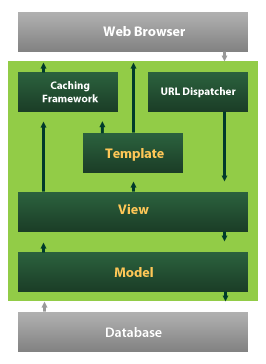
\includegraphics[width=0.4\textwidth]{figures/chapter5/Django_mvc.png}
    \caption[Model Template View - MTV]{Model View Template, Fuente: \url{http://djangoproject.org}}
  \end{center}
\end{figure}

Ahora llegamos a la pregunta ¿dónde viene a encajar el {\it ``controlador''}? En el caso
de Django, es probable que sea el Framework en si. La maquina que envía una
solicitud a la vista apropiada, de acuerdo con la configuración de los URL de Django
y las que definimos en nuestro proyecto que se encuentran en ``{\it urls.py}''.

Para entender a detalle este flujo que sigue Django tenemos la siguiente figura.

\begin{figure}[h]
  \begin{center}
    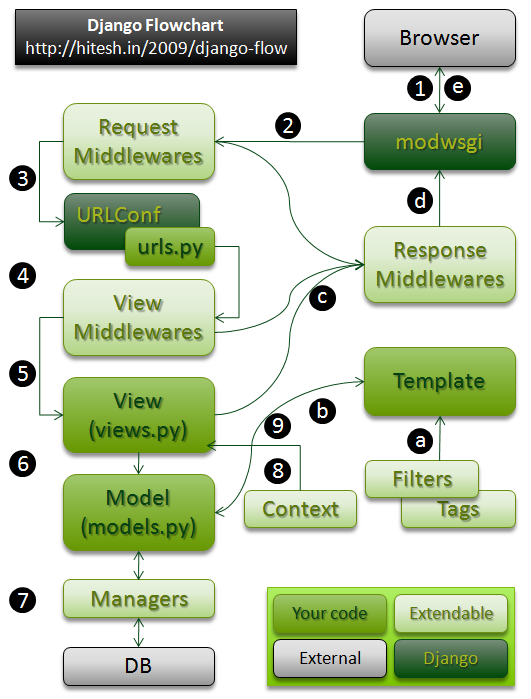
\includegraphics[width=0.6\textwidth]{figures/chapter5/DjangoFlow.png}
    \caption[El flujo de Django]{Una vista general del flujo de Django, Fuente: \url{http://hitesh.in/2009/django-flow/}}
  \end{center}
\end{figure}

\newpage

\begin{enumerate}
    \item El usuario hace una solicitud de una pagina.
    \item La solicitud llega a un {\it Request Middlewares} el cual lo manipula o
      responde a la solicitud.
    \item El {\it URLConf} busca la vista relacionada usando los {\it urls.py}
    \item {\it View Middlewares} es llamado, que manipula o responde a la
      solicitud.
    \item La función {\it view} es invocada.
    \item La vista puede opcionalmente tener acceso a los datos a través de los
        modelos.
    \item Todas las interacciones de modelo-a-DB se hacen a través de un {\it manager}.
    \item Las vistas podrían usar un {\it context} especial si es necesario.
    \item El context se pasa al {\it template} para la presentación.
\end{enumerate}

\begin{itemize}
  \item[a] Los templates usan {\it Filters} y {\it Tags} para la salida de la presentación.
  \item[b] La salida devuelta a la vista.
  \item[c] {\it HTTPResponse} envía a {\it Response Middlerwares}.
  \item[d] Cada una de las respuestas de los {\it Middlewares} puede enriquecer
    la respuesta o devolver completamente una nueva respuesta.
  \item[e] La respuesta es enviada la navegador del usuario.
\end{itemize}

\section{Estructura del Proyecto}
Ya con una vista general de como funciona Django vamos a ver como se estructura
un proyecto en Django.

\begin{verbatim}
flosite
    |-- manage.py
    |-- flosite (carpeta principal)
    |   |-- __init__.py
    |   |-- settings.py (archivo de Configuración del proyecto)
    |   |-- urls.py (urls que direcciona a las urls de las apps)
    |   `-- wsgi.py
    `-- app_one
    |   |-- templates/ (templates para el uso de este app)
    |   |-- __init__.py
    |   |-- models.py
    |   |-- views.py
    |   `-- urls.py (url que direcciona a las views de esta app)
    `-- app_two
    |   |-- templates/
    |   |-- __init__.py
    |   |-- models.py
    |   |-- views.py
    |   `-- urls.py
    `-- templates (Templates para el uso general del proyecto)
    |   |-- base.html
    |   |-- index.html
    `-- staticfiles
        |-- css/
        `-- js/

\end{verbatim}

Nuestro proyecto {\it flosite} cuenta con ocho aplicaciones, como ser: {\it account,
branchoffice, core, guest, maintenance, notifications, register, staff}. Algo
que es importante mencionar es que desde la versión 1.4 de Django los templates
se manejan diferente, ya que se tiene una carpeta {\it templates} para el uso
general del proyecto y cada aplicación maneja su propia carpeta de {\it templates}.

\begin{figure}[h]
  \begin{center}
    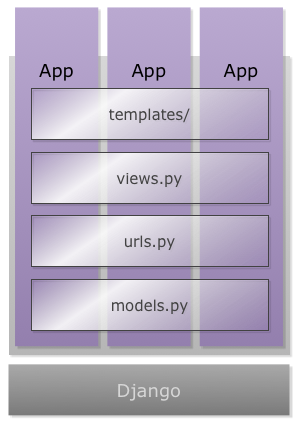
\includegraphics[width=0.3\textwidth]{figures/chapter5/appsdjango2.png}
    \caption[Estructura de una aplicación de un proyecto Django]{Estructura de una aplicación de un proyecto Django}
  \end{center}
\end{figure}

El archivo {\it flosite/urls.py} es muy importante que este bien configurado, ya
que este se encarga de delegar las peticiones que se hacen a las aplicaciones
correspondientes

\begin{verbatim}
$ less flosite/urls.py
\end{verbatim}

\newpage

{\scriptsize
\begin{verbatim}
from django.conf.urls import patterns, include, url
from django.views.generic import TemplateView
from django.conf import settings
from django.conf.urls.static import static
from django.contrib.staticfiles.urls import staticfiles_urlpatterns

from django.contrib import admin
admin.autodiscover()

urlpatterns = patterns('',
    url(r'^$', TemplateView.as_view(template_name='index.html'), name="home"),
    url(r'^accounts/', include('userena.urls')),
    url(r'^messages/', include('userena.contrib.umessages.urls')),
    url(r'^staff/', include('staff.urls')),
    url(r'^branchoffice/', include('branchoffice.urls')),
    url(r'^notifications/', include('notifications.urls')),
    url(r'^maintenance/', include('maintenance.urls')),
    url(r'^guest/', include('guest.urls')),
    url(r'^register/', include('register.urls')),
    url(r'^admin/', include(admin.site.urls)),
) + static(settings.MEDIA_URL, document_root=settings.MEDIA_ROOT)

urlpatterns += staticfiles_urlpatterns()
\end{verbatim}
}

Gráficamente tendríamos lo siguiente:

\begin{figure}[h]
  \begin{center}
    \def\svgwidth{\columnwidth}
    \input{figures/chapter5/urls.pdf_tex}
    \caption[Django Urls]{flosite/urls.py}
  \end{center}
\end{figure}

\section{Configuración del proyecto}
La configuración del proyecto se encuentra en {\it flosite/settings.py}, no
mostraremos todo el archivo de configuración solo resaltaremos las partes más
importantes.

\subsection{El archivo settings.py}
Al crear un proyecto con Django\footnote{Vea el apéndice de Instalación para
más detalles} se crea un archivo settings.py donde uno tiene que modificar el
archivo con los datos correspondientes.

\begin{verbatim}
$ less flosite/settings.py
\end{verbatim}

\begin{verbatim}
DATABASES = {
    'default': {
         # Add 'postgresql_psycopg2', 'mysql', 'sqlite3' or 'oracle'.
        'ENGINE': 'django.db.backends.mysql',
        'NAME': 'nombre_base_de_datos',
        'USER': '#########',
        'PASSWORD': '############',
        'HOST': '',
        'PORT': '', # Set to empty string for default.
    }
}
\end{verbatim}

Para instalar las aplicaciones que hemos creado en el archivo {\it settings.py}
se tiene otra sección especifica para esto:

\begin{verbatim}
INSTALLED_APPS = (
    # default
    'django.contrib.auth',
    'django.contrib.contenttypes',
    'django.contrib.sessions',
    'django.contrib.sites',
    'django.contrib.messages',
    'django.contrib.staticfiles',

    # ....

    # project flosite
    'accounts',
    'staff',
    'guest',
    'branchoffice',
    'guest',
    'register',
    'core',
    'notifications',
    'maintenance',
\end{verbatim}

Todas las aplicaciones que se mencionan en esta sección son las que se instalan
al momento de hacer un {\it syncdb}.\footnote{Vea el apéndice de Instalación para
mas detalles}

\begin{verbatim}
$ python manage.py syncdb
\end{verbatim}

\section{Aplicaciones extras para el sistema}
Teniendo en cuenta las herramientas y bondades que ofrece Django, para el proyecto
usamos las siguientes aplicaciones ya desarrolladas.

\begin{verbatim}
INSTALLED_APPS = (
    # ....

    #extras
    'bootstrap_toolkit',
    'bootstrap3_datetime',
    'pagination',
    'debug_toolbar',
    'userena',

  # ....
)
\end{verbatim}

\begin{itemize}
    \item bootstrap\_toolkit: nos ofrece todo el diseño web y paginas de estilo
      necesarias.
    \item bootstrap3\_datetime: nos permite el manejo de calendarios en los forms.
    \item pagination: Esta herramienta es muy importante para la paginación de tablas.
    \item debug\_toolbar: Una herramienta útil para debug.
    \item userena: Para el manejo de usuarios y sus perfiles.
\end{itemize}

\begin{figure}[h]
  \begin{center}
    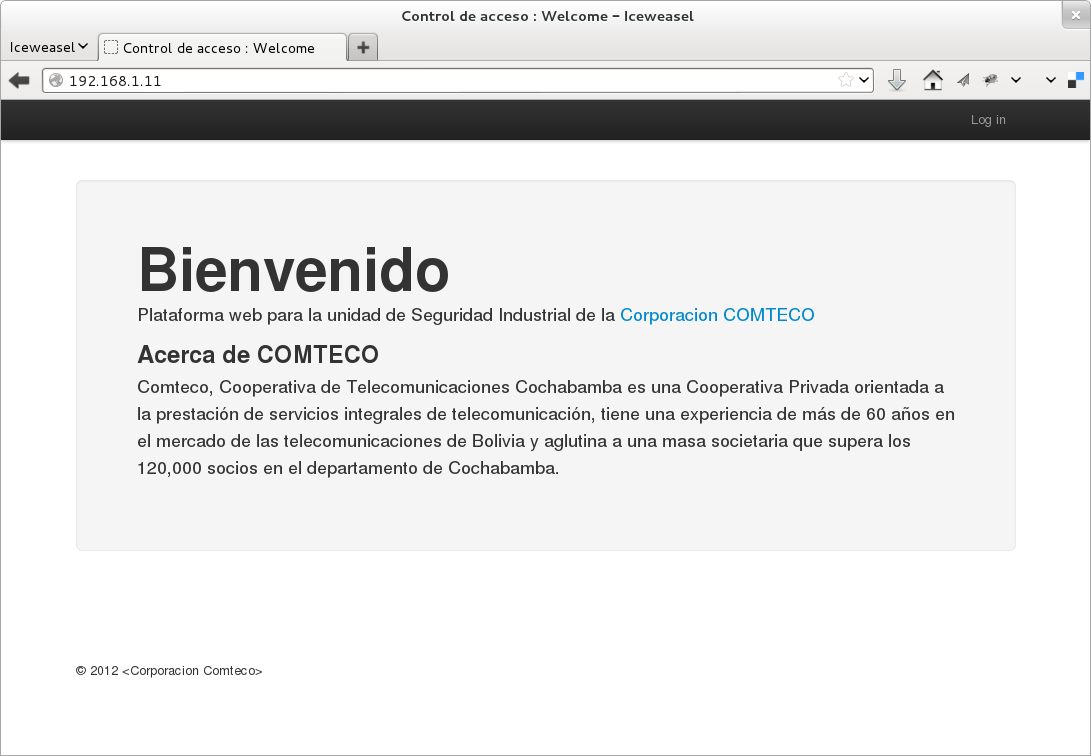
\includegraphics[width=0.6\textwidth]{figures/chapter5/homepage.png}
    \caption[Página de inicio del Sistema Web]{Página de inicio del Sistema Web}
  \end{center}
\end{figure}

\section{Formularios para los registros}
Para el sistema tenemos tres formularios: {\it Registro de vehículos, Registro
de Personas, Reportes}

\subsection{Registro de Vehículos}
Los formularios para los registro se encuentra en {\it register/forms.py}

\begin{verbatim}
$ less register/forms.py
\end{verbatim}

\begin{verbatim}
from django import forms

class RegisterKmForm(forms.Form):
    r_automotive = forms.CharField(widget=forms.TextInput(attrs={...}))
    r_km_revert = forms.BooleanField(required=False)
    r_date   = forms.DateField(widget=BootstrapDateInput(attrs={...}))
    r_hour   = forms.TimeField(widget=forms.TextInput(attrs={...}))
    r_km     = forms.IntegerField(label=_('output_km'), widget=...)
    r_driver = forms.CharField(widget=forms.TextInput(attrs={...}))
    r_ladder = forms.CharField(required=False)
    r_obs    = forms.CharField(widget=forms.Textarea, required=False)

    # validators
    def ...
\end{verbatim}
A estos formularios se los llama desde {\it register/views.py} y lo carga en el
template {\it register/templates/register\_form.html} para tener el siguiente
formulario:

El código de {\it views.py} para registro de vehículos seria el siguiente:

\begin{alltt}
from django.shortcuts import render, ...
from register.forms import \emph{RegisterKmForm}, ...

@login_required
@csrf_protect
@permission_required_or_403('register.add_register_automotive')
def form_car(request):
    ....
    if request.method == 'POST':
        form = \emph{RegisterKmForm(request.POST)} # Esta linea llama al form
        if form.is_valid():
            ....
    else:
      form = \emph{RegisterKmForm()}
    return render(request, 'register_form.html', {'form': form})
\end{alltt}

La ultima linea es la que se encarga principalmente de renderizar el template con
el formulario.

\begin{verbatim}
return render(request, 'register_form.html', {'form': form})
\end{verbatim}

Y con todo, tendríamos la siguiente vista:

\begin{figure}[h]
  \begin{center}
    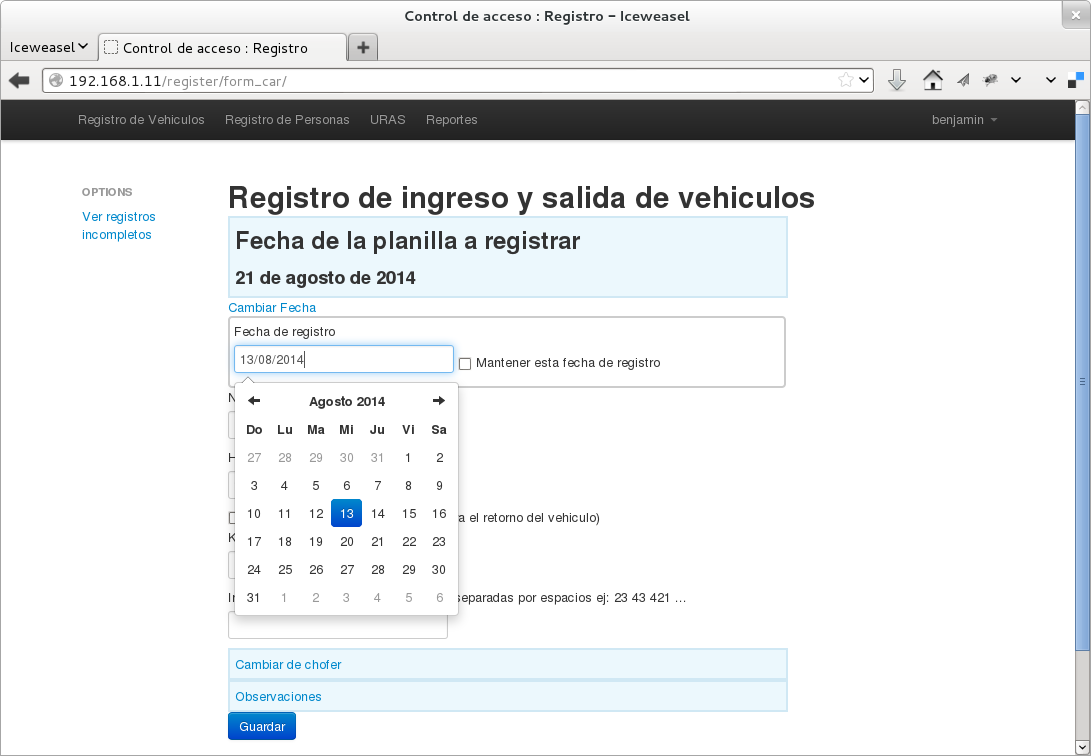
\includegraphics[width=0.8\textwidth]{figures/chapter5/registro2.png}
    \caption[Formulario de Registro de Vehículos]{Formulario de Registro de Vehículo}
  \end{center}
\end{figure}

\newpage

\subsection{Registro de Personas}
El formulario para el registro de personas se encuentra también en {\it register/forms.py}
y seria el siguiente:

\begin{verbatim}
class RegisterPersonForm(forms.Form):
    LOCALE_CHOICES = (
        ('cba', 'Cochabamba'),
        ('lpz', 'La Paz'),
        ('scz', 'Santa Cruz'),
        ('pnd', 'Pando'),
        ('ben', 'Beni'),
        ('oru', 'Oruro'),
        ('pts', 'Potosi'),
        ('tja', 'Tarija'),
        ('scr', 'Chuquisaca'),
        ('---', _('none')),
        )

    GENDER_CHOICES = (
        ('H', 'Hombre'),
        ('M', 'Mujer')
    )
    identity_document = forms.CharField(required=True, widget=...)
    city = forms.CharField(required=True, widget=forms.Select(...))
    first_name = forms.CharField(required=True)
    last_name = forms.CharField(required=True)
    gender = forms.CharField(required=True, widget=forms.Select(...))
    reason = forms.CharField(required=True, widget=forms.Textarea)
\end{verbatim}

La llamada desde el {\it views.py}

\begin{alltt}

from register.forms import RegisterPersonForm

@login_required
@csrf_protect
@permission_required_or_403('register.add_register_person')
def form_register_person(request):
    if request.method == 'POST':
        form = \emph{RegisterPersonForm(request.POST)}
        if form.is_valid():
            ...
            return HttpResponseRedirect('/register/persons')
    else:
        form  = \emph{RegisterPersonForm()}
    return render(request, 'form_register_person.html', {'form': form})
\end{alltt}

Esta vista llama al template {\it form\_register\_person.html}

\begin{figure}[h]
  \begin{center}
    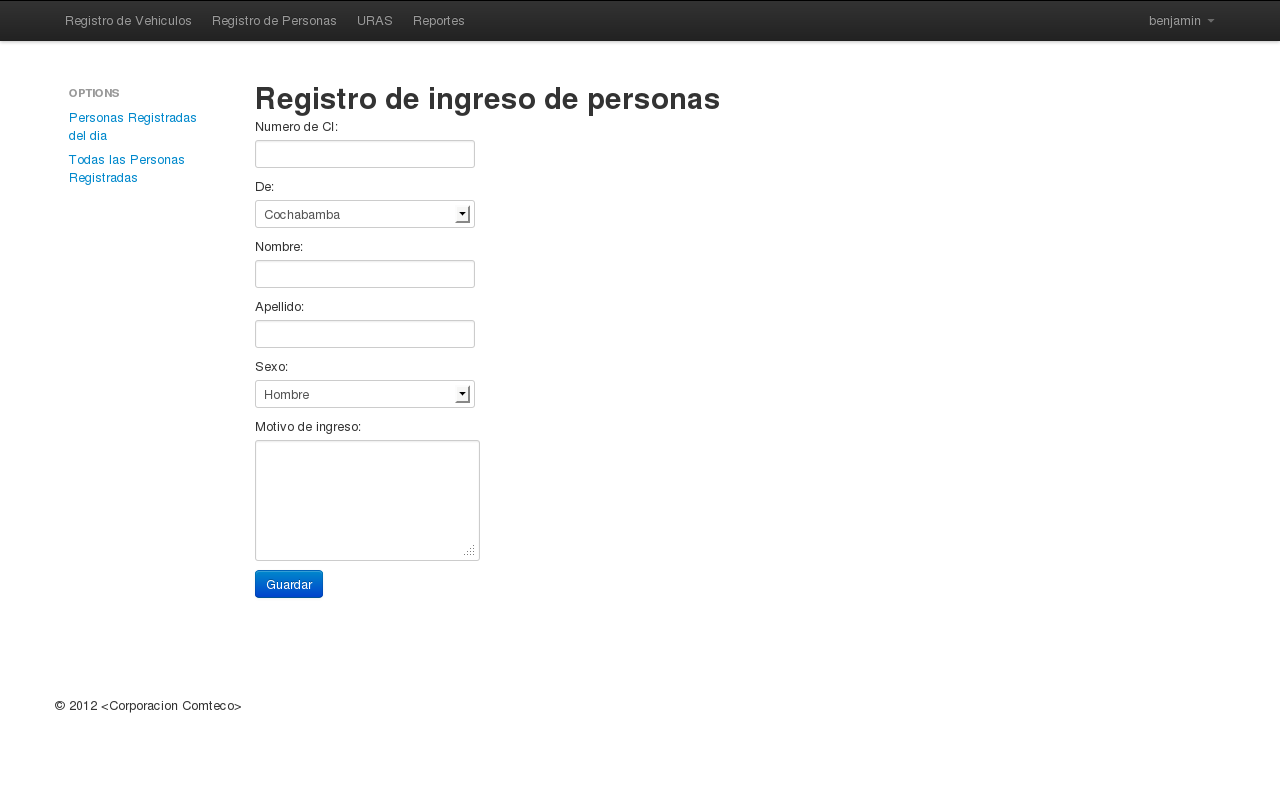
\includegraphics[width=0.8\textwidth]{figures/chapter5/registro_personas.png}
    \caption[Formulario de Registro de Personas]{Formulario para el Registro de Personas}
  \end{center}
\end{figure}

\newpage

\subsection{Reportes}
El formulario para los reportes se encuentra {\it report/forms.py}

\begin{verbatim}
class ReportForm(forms.Form):
    generate_pdf = forms.BooleanField(required=False)
    generate_excel = forms.BooleanField(required=False)
    parking = forms.ModelChoiceField(queryset=LocaleParking.objects.all(),
                                     empty_label="(seleccione un parqueo)")
    today = forms.DateField(label='today', widget=BootstrapDateInput(...))
    date_begin = forms.DateField(widget=BootstrapDateInput(...)
    date_end = forms.DateField(widget=BootstrapDateInput(format="%d/%m/%Y"), ..)
    internal_num_car = forms.CharField(max_length=10, required=False)
    item_driver = forms.CharField(max_length=10, required=False)
\end{verbatim}

La llamada desde el vista es la siguiente y se encuentra en {\it report/views.py}

\begin{alltt}
@login_required
def home(request):
    if 'csrfmiddlewaretoken' in request.GET:
        form = \emph{ReportForm(request.GET)}
        if form.is\_valid():
            .....
    else:
        return render\_to\_response('report/list.html', {'report': report.order\_by(...)})
    else:
        form = \emph{ReportForm()}

    return render(request, 'report/report.html', {'form': form})
\end{alltt}

Esta vista llama al template {\it report/report.html}

\begin{figure}[h]
  \begin{center}
    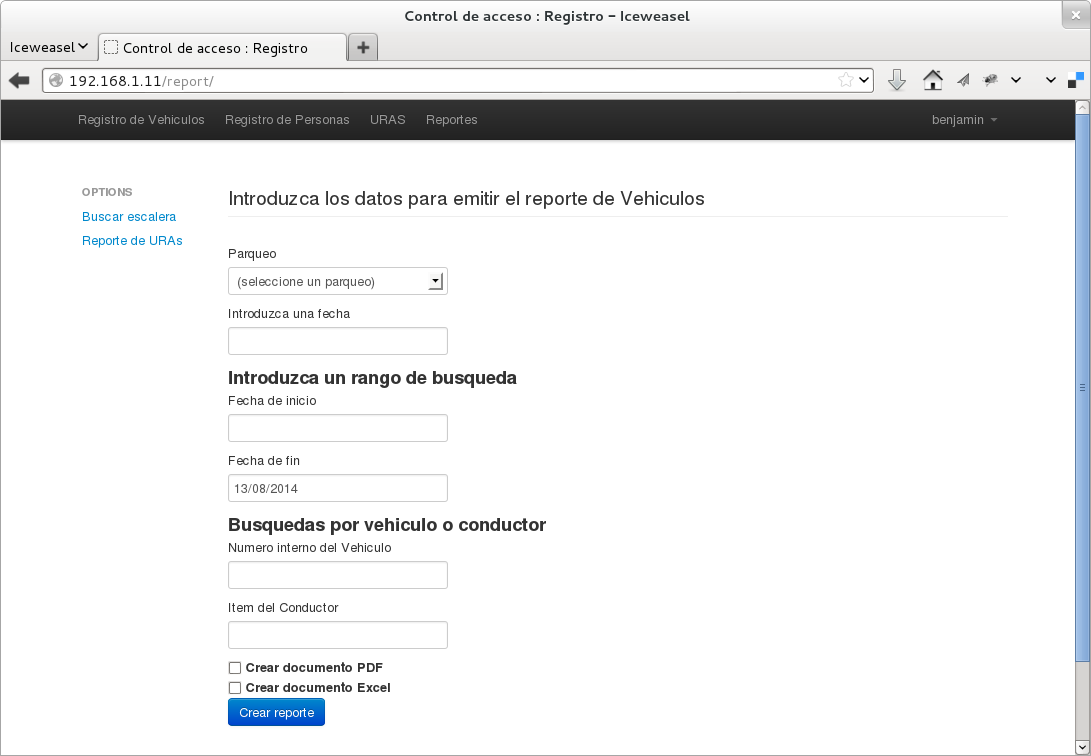
\includegraphics[width=0.8\textwidth]{figures/chapter5/reportes.png}
    \caption[Formulario para Reportes]{Formulario para Reportes}
  \end{center}
\end{figure}

